\documentclass[twoside]{book}

% Packages required by doxygen
\usepackage{fixltx2e}
\usepackage{calc}
\usepackage{doxygen}
\usepackage[export]{adjustbox} % also loads graphicx
\usepackage{graphicx}
\usepackage[utf8]{inputenc}
\usepackage{makeidx}
\usepackage{multicol}
\usepackage{multirow}
\PassOptionsToPackage{warn}{textcomp}
\usepackage{textcomp}
\usepackage[nointegrals]{wasysym}
\usepackage[table]{xcolor}

% Font selection
\usepackage[T1]{fontenc}
\usepackage[scaled=.90]{helvet}
\usepackage{courier}
\usepackage{amssymb}
\usepackage{sectsty}
\renewcommand{\familydefault}{\sfdefault}
\allsectionsfont{%
  \fontseries{bc}\selectfont%
  \color{darkgray}%
}
\renewcommand{\DoxyLabelFont}{%
  \fontseries{bc}\selectfont%
  \color{darkgray}%
}
\newcommand{\+}{\discretionary{\mbox{\scriptsize$\hookleftarrow$}}{}{}}

% Page & text layout
\usepackage{geometry}
\geometry{%
  a4paper,%
  top=2.5cm,%
  bottom=2.5cm,%
  left=2.5cm,%
  right=2.5cm%
}
\tolerance=750
\hfuzz=15pt
\hbadness=750
\setlength{\emergencystretch}{15pt}
\setlength{\parindent}{0cm}
\setlength{\parskip}{3ex plus 2ex minus 2ex}
\makeatletter
\renewcommand{\paragraph}{%
  \@startsection{paragraph}{4}{0ex}{-1.0ex}{1.0ex}{%
    \normalfont\normalsize\bfseries\SS@parafont%
  }%
}
\renewcommand{\subparagraph}{%
  \@startsection{subparagraph}{5}{0ex}{-1.0ex}{1.0ex}{%
    \normalfont\normalsize\bfseries\SS@subparafont%
  }%
}
\makeatother

% Headers & footers
\usepackage{fancyhdr}
\pagestyle{fancyplain}
\fancyhead[LE]{\fancyplain{}{\bfseries\thepage}}
\fancyhead[CE]{\fancyplain{}{}}
\fancyhead[RE]{\fancyplain{}{\bfseries\leftmark}}
\fancyhead[LO]{\fancyplain{}{\bfseries\rightmark}}
\fancyhead[CO]{\fancyplain{}{}}
\fancyhead[RO]{\fancyplain{}{\bfseries\thepage}}
\fancyfoot[LE]{\fancyplain{}{}}
\fancyfoot[CE]{\fancyplain{}{}}
\fancyfoot[RE]{\fancyplain{}{\bfseries\scriptsize Generated by Doxygen }}
\fancyfoot[LO]{\fancyplain{}{\bfseries\scriptsize Generated by Doxygen }}
\fancyfoot[CO]{\fancyplain{}{}}
\fancyfoot[RO]{\fancyplain{}{}}
\renewcommand{\footrulewidth}{0.4pt}
\renewcommand{\chaptermark}[1]{%
  \markboth{#1}{}%
}
\renewcommand{\sectionmark}[1]{%
  \markright{\thesection\ #1}%
}

% Indices & bibliography
\usepackage{natbib}
\usepackage[titles]{tocloft}
\setcounter{tocdepth}{3}
\setcounter{secnumdepth}{5}
\makeindex

% Hyperlinks (required, but should be loaded last)
\usepackage{ifpdf}
\ifpdf
  \usepackage[pdftex,pagebackref=true]{hyperref}
\else
  \usepackage[ps2pdf,pagebackref=true]{hyperref}
\fi
\hypersetup{%
  colorlinks=true,%
  linkcolor=blue,%
  citecolor=blue,%
  unicode%
}

% Custom commands
\newcommand{\clearemptydoublepage}{%
  \newpage{\pagestyle{empty}\cleardoublepage}%
}

\usepackage{caption}
\captionsetup{labelsep=space,justification=centering,font={bf},singlelinecheck=off,skip=4pt,position=top}

%===== C O N T E N T S =====

\begin{document}

% Titlepage & ToC
\hypersetup{pageanchor=false,
             bookmarksnumbered=true,
             pdfencoding=unicode
            }
\pagenumbering{alph}
\begin{titlepage}
\vspace*{7cm}
\begin{center}%
{\Large Runaway from hell }\\
\vspace*{1cm}
{\large Generated by Doxygen 1.8.12}\\
\end{center}
\end{titlepage}
\clearemptydoublepage
\pagenumbering{roman}
\tableofcontents
\clearemptydoublepage
\pagenumbering{arabic}
\hypersetup{pageanchor=true}

%--- Begin generated contents ---
\chapter{Hierarchical Index}
\section{Class Hierarchy}
This inheritance list is sorted roughly, but not completely, alphabetically\+:\begin{DoxyCompactList}
\item Mono\+Behaviour\begin{DoxyCompactList}
\item \contentsline{section}{Camera\+Controll}{\pageref{class_camera_controll}}{}
\item \contentsline{section}{Dead\+And\+Restart}{\pageref{class_dead_and_restart}}{}
\item \contentsline{section}{Dead\+Menu}{\pageref{class_dead_menu}}{}
\item \contentsline{section}{Destroyer}{\pageref{class_destroyer}}{}
\item \contentsline{section}{Main\+Menu}{\pageref{class_main_menu}}{}
\item \contentsline{section}{Obstacle}{\pageref{class_obstacle}}{}
\item \contentsline{section}{Obstacle\+Controller}{\pageref{class_obstacle_controller}}{}
\item \contentsline{section}{Pause\+Menu}{\pageref{class_pause_menu}}{}
\item \contentsline{section}{Platform\+Generator}{\pageref{class_platform_generator}}{}
\item \contentsline{section}{Player\+Controller}{\pageref{class_player_controller}}{}
\item \contentsline{section}{Score\+Controller}{\pageref{class_score_controller}}{}
\end{DoxyCompactList}
\item \contentsline{section}{Object\+Destroyer}{\pageref{interface_object_destroyer}}{}
\end{DoxyCompactList}

\chapter{Class Index}
\section{Class List}
Here are the classes, structs, unions and interfaces with brief descriptions\+:\begin{DoxyCompactList}
\item\contentsline{section}{\hyperlink{class_camera_controll}{Camera\+Controll} }{\pageref{class_camera_controll}}{}
\item\contentsline{section}{\hyperlink{class_dead_and_restart}{Dead\+And\+Restart} }{\pageref{class_dead_and_restart}}{}
\item\contentsline{section}{\hyperlink{class_dead_menu}{Dead\+Menu} }{\pageref{class_dead_menu}}{}
\item\contentsline{section}{\hyperlink{class_destroyer}{Destroyer} }{\pageref{class_destroyer}}{}
\item\contentsline{section}{\hyperlink{class_main_menu}{Main\+Menu} }{\pageref{class_main_menu}}{}
\item\contentsline{section}{\hyperlink{interface_object_destroyer}{Object\+Destroyer} }{\pageref{interface_object_destroyer}}{}
\item\contentsline{section}{\hyperlink{class_obstacle}{Obstacle} }{\pageref{class_obstacle}}{}
\item\contentsline{section}{\hyperlink{class_obstacle_controller}{Obstacle\+Controller} }{\pageref{class_obstacle_controller}}{}
\item\contentsline{section}{\hyperlink{class_pause_menu}{Pause\+Menu} }{\pageref{class_pause_menu}}{}
\item\contentsline{section}{\hyperlink{class_platform_generator}{Platform\+Generator} }{\pageref{class_platform_generator}}{}
\item\contentsline{section}{\hyperlink{class_player_controller}{Player\+Controller} }{\pageref{class_player_controller}}{}
\item\contentsline{section}{\hyperlink{class_score_controller}{Score\+Controller} }{\pageref{class_score_controller}}{}
\end{DoxyCompactList}

\chapter{Class Documentation}
\hypertarget{class_camera_controll}{}\section{Camera\+Controll Class Reference}
\label{class_camera_controll}\index{Camera\+Controll@{Camera\+Controll}}
Inheritance diagram for Camera\+Controll\+:\begin{figure}[H]
\begin{center}
\leavevmode
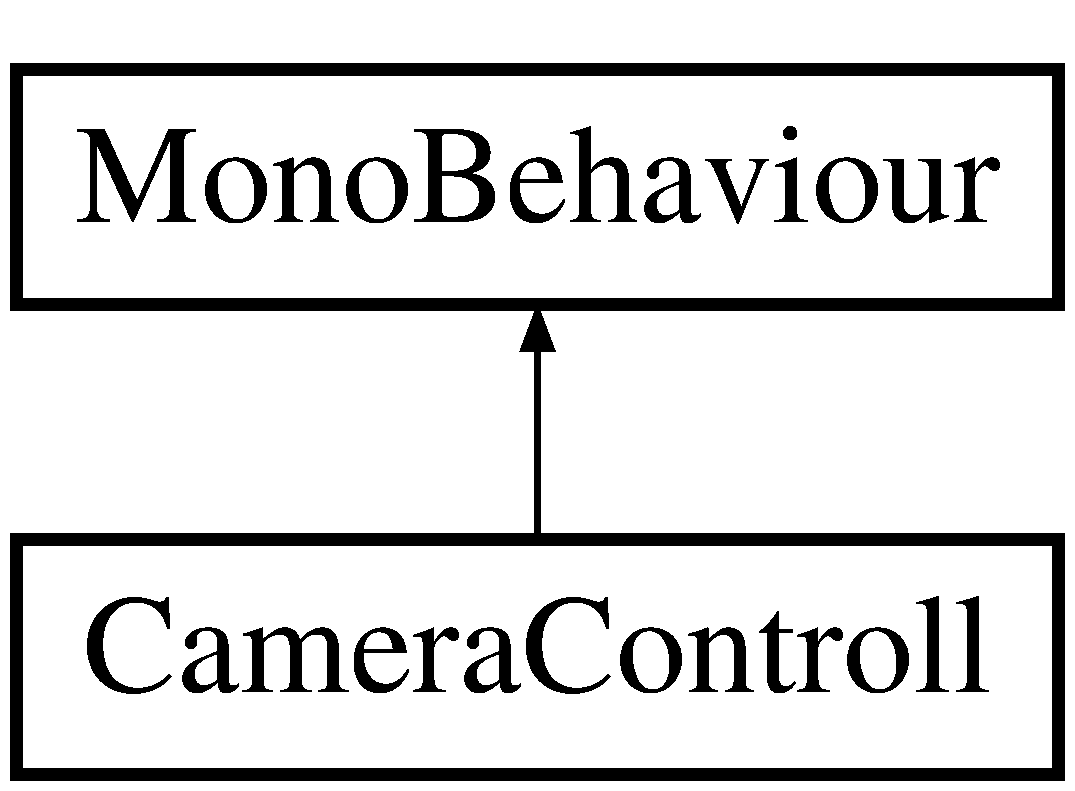
\includegraphics[height=2.000000cm]{class_camera_controll}
\end{center}
\end{figure}
\subsection*{Public Attributes}
\begin{DoxyCompactItemize}
\item 
\hypertarget{class_camera_controll_aaf8cb2822b242349a0d58e22da4d8bd8}{}\label{class_camera_controll_aaf8cb2822b242349a0d58e22da4d8bd8} 
\hyperlink{class_player_controller}{Player\+Controller} {\bfseries the\+Player}
\end{DoxyCompactItemize}
\subsection*{Private Member Functions}
\begin{DoxyCompactItemize}
\item 
\hypertarget{class_camera_controll_ac798631e3e2fe815a27e363c1c4423dd}{}\label{class_camera_controll_ac798631e3e2fe815a27e363c1c4423dd} 
void \hyperlink{class_camera_controll_ac798631e3e2fe815a27e363c1c4423dd}{Start} ()
\begin{DoxyCompactList}\small\item\em Use this for initialization. \end{DoxyCompactList}\item 
void \hyperlink{class_camera_controll_a79756d5ea4d853ab67752d483395b192}{Update} ()
\begin{DoxyCompactList}\small\item\em method ini akan membuat kamera mengikuti gerakan player saat bergerak dan akan tetap stibil di tengah walaupun player melompat \end{DoxyCompactList}\end{DoxyCompactItemize}
\subsection*{Private Attributes}
\begin{DoxyCompactItemize}
\item 
\hypertarget{class_camera_controll_a811a96b63a2b0fde284a7b6bad4c1c17}{}\label{class_camera_controll_a811a96b63a2b0fde284a7b6bad4c1c17} 
Vector3 {\bfseries last\+Player\+Position}
\item 
\hypertarget{class_camera_controll_a8ede8e227ec5e447b031d1321e2a991c}{}\label{class_camera_controll_a8ede8e227ec5e447b031d1321e2a991c} 
float {\bfseries distance\+To\+Move}
\end{DoxyCompactItemize}


\subsection{Member Function Documentation}
\hypertarget{class_camera_controll_a79756d5ea4d853ab67752d483395b192}{}\label{class_camera_controll_a79756d5ea4d853ab67752d483395b192} 
\index{Camera\+Controll@{Camera\+Controll}!Update@{Update}}
\index{Update@{Update}!Camera\+Controll@{Camera\+Controll}}
\subsubsection{\texorpdfstring{Update()}{Update()}}
{\footnotesize\ttfamily void Camera\+Controll.\+Update (\begin{DoxyParamCaption}{ }\end{DoxyParamCaption})\hspace{0.3cm}{\ttfamily [private]}}



method ini akan membuat kamera mengikuti gerakan player saat bergerak dan akan tetap stibil di tengah walaupun player melompat 



The documentation for this class was generated from the following file\+:\begin{DoxyCompactItemize}
\item 
C\+:/\+Users/\+Irvan/\+Documents/\+Git\+Hub/\+Tugas\+Akhir\+A\+D\+B\+O/game fix/\+Endless\+Runner/\+Assets/\+Script/Camera\+Controll.\+cs\end{DoxyCompactItemize}

\hypertarget{class_dead_and_restart}{}\section{Dead\+And\+Restart Class Reference}
\label{class_dead_and_restart}\index{Dead\+And\+Restart@{Dead\+And\+Restart}}
Inheritance diagram for Dead\+And\+Restart\+:\begin{figure}[H]
\begin{center}
\leavevmode
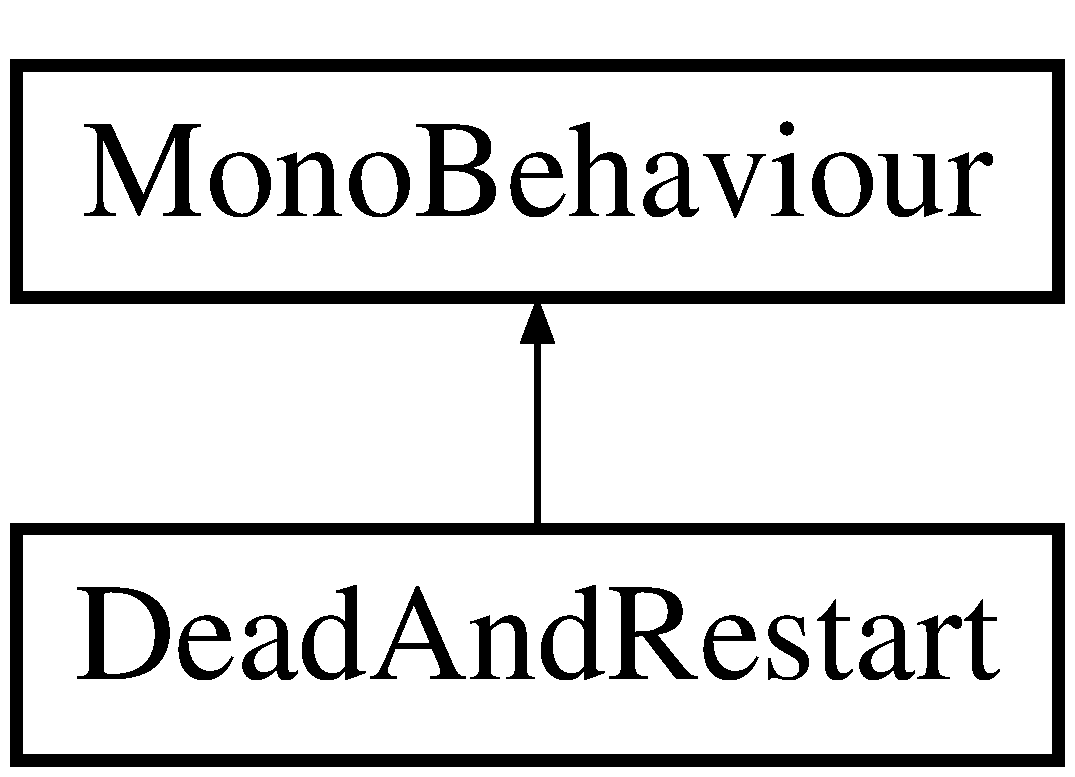
\includegraphics[height=2.000000cm]{class_dead_and_restart}
\end{center}
\end{figure}
\subsection*{Public Member Functions}
\begin{DoxyCompactItemize}
\item 
void \hyperlink{class_dead_and_restart_a051bee469f462b949f4ce83791c2294f}{kill\+The\+Player} ()
\begin{DoxyCompactList}\small\item\em method ini akan menghilankan player saat mati sehingga tidak ada dalam platform dan saat bersamaan akan memanggil tampilan dari \hyperlink{class_dead_menu}{Dead\+Menu} \end{DoxyCompactList}\item 
void \hyperlink{class_dead_and_restart_a38d762c09b1bcaa35a0a2cb0807c38f3}{reset} ()
\begin{DoxyCompactList}\small\item\em saat dipanggil akan \hyperlink{class_dead_menu}{Dead\+Menu} akan ditutup dan akan mengulang semua arena dari awal \end{DoxyCompactList}\end{DoxyCompactItemize}
\subsection*{Public Attributes}
\begin{DoxyCompactItemize}
\item 
\hypertarget{class_dead_and_restart_a7700d89251ec094e373a0fe7e61f09f9}{}\label{class_dead_and_restart_a7700d89251ec094e373a0fe7e61f09f9} 
Transform {\bfseries platform\+Generator}
\item 
\hypertarget{class_dead_and_restart_aba66184a8d37c05c78f86e2c83628eae}{}\label{class_dead_and_restart_aba66184a8d37c05c78f86e2c83628eae} 
\hyperlink{class_player_controller}{Player\+Controller} {\bfseries the\+Player}
\item 
\hypertarget{class_dead_and_restart_a855a9b0c48730b94b800589d74d887ae}{}\label{class_dead_and_restart_a855a9b0c48730b94b800589d74d887ae} 
\hyperlink{class_dead_menu}{Dead\+Menu} {\bfseries dead\+Menu\+Screen}
\item 
\hypertarget{class_dead_and_restart_a68ea47d86cdc8884858f2951ae90c063}{}\label{class_dead_and_restart_a68ea47d86cdc8884858f2951ae90c063} 
Audio\+Source {\bfseries death\+Sound\+Effect}
\end{DoxyCompactItemize}
\subsection*{Private Member Functions}
\begin{DoxyCompactItemize}
\item 
void \hyperlink{class_dead_and_restart_ace49e4505012656acdfdf947e22cfaab}{Start} ()
\begin{DoxyCompactList}\small\item\em method ini akan menyimpan letak awal platform dan player; \end{DoxyCompactList}\end{DoxyCompactItemize}
\subsection*{Private Attributes}
\begin{DoxyCompactItemize}
\item 
\hypertarget{class_dead_and_restart_ad88cf9f54b6f7ab52dcfb9231c2e881d}{}\label{class_dead_and_restart_ad88cf9f54b6f7ab52dcfb9231c2e881d} 
Vector3 {\bfseries platform\+Start\+Point}
\item 
\hypertarget{class_dead_and_restart_a5fc332be57d38f79d00e1f59c3e1fec0}{}\label{class_dead_and_restart_a5fc332be57d38f79d00e1f59c3e1fec0} 
Vector3 {\bfseries player\+Start\+Point}
\item 
\hypertarget{class_dead_and_restart_add548a0fec72d4ddd716e4769f99ecd7}{}\label{class_dead_and_restart_add548a0fec72d4ddd716e4769f99ecd7} 
\hyperlink{class_obstacle_controller}{Obstacle\+Controller} {\bfseries obs\+Controller}
\item 
\hypertarget{class_dead_and_restart_ad4a397b1236d0a27ad6b96daf7421064}{}\label{class_dead_and_restart_ad4a397b1236d0a27ad6b96daf7421064} 
\hyperlink{class_destroyer}{Destroyer} \mbox{[}$\,$\mbox{]} {\bfseries list}
\end{DoxyCompactItemize}


\subsection{Member Function Documentation}
\hypertarget{class_dead_and_restart_a051bee469f462b949f4ce83791c2294f}{}\label{class_dead_and_restart_a051bee469f462b949f4ce83791c2294f} 
\index{Dead\+And\+Restart@{Dead\+And\+Restart}!kill\+The\+Player@{kill\+The\+Player}}
\index{kill\+The\+Player@{kill\+The\+Player}!Dead\+And\+Restart@{Dead\+And\+Restart}}
\subsubsection{\texorpdfstring{kill\+The\+Player()}{killThePlayer()}}
{\footnotesize\ttfamily void Dead\+And\+Restart.\+kill\+The\+Player (\begin{DoxyParamCaption}{ }\end{DoxyParamCaption})}



method ini akan menghilankan player saat mati sehingga tidak ada dalam platform dan saat bersamaan akan memanggil tampilan dari \hyperlink{class_dead_menu}{Dead\+Menu} 

\hypertarget{class_dead_and_restart_a38d762c09b1bcaa35a0a2cb0807c38f3}{}\label{class_dead_and_restart_a38d762c09b1bcaa35a0a2cb0807c38f3} 
\index{Dead\+And\+Restart@{Dead\+And\+Restart}!reset@{reset}}
\index{reset@{reset}!Dead\+And\+Restart@{Dead\+And\+Restart}}
\subsubsection{\texorpdfstring{reset()}{reset()}}
{\footnotesize\ttfamily void Dead\+And\+Restart.\+reset (\begin{DoxyParamCaption}{ }\end{DoxyParamCaption})}



saat dipanggil akan \hyperlink{class_dead_menu}{Dead\+Menu} akan ditutup dan akan mengulang semua arena dari awal 

\hypertarget{class_dead_and_restart_ace49e4505012656acdfdf947e22cfaab}{}\label{class_dead_and_restart_ace49e4505012656acdfdf947e22cfaab} 
\index{Dead\+And\+Restart@{Dead\+And\+Restart}!Start@{Start}}
\index{Start@{Start}!Dead\+And\+Restart@{Dead\+And\+Restart}}
\subsubsection{\texorpdfstring{Start()}{Start()}}
{\footnotesize\ttfamily void Dead\+And\+Restart.\+Start (\begin{DoxyParamCaption}{ }\end{DoxyParamCaption})\hspace{0.3cm}{\ttfamily [private]}}



method ini akan menyimpan letak awal platform dan player; 



The documentation for this class was generated from the following file\+:\begin{DoxyCompactItemize}
\item 
C\+:/\+Users/\+Irvan/\+Documents/\+Git\+Hub/\+Tugas\+Akhir\+A\+D\+B\+O/game fix/\+Endless\+Runner/\+Assets/\+Script/Dead\+And\+Restart.\+cs\end{DoxyCompactItemize}

\hypertarget{class_dead_menu}{}\section{Dead\+Menu Class Reference}
\label{class_dead_menu}\index{Dead\+Menu@{Dead\+Menu}}
Inheritance diagram for Dead\+Menu\+:\begin{figure}[H]
\begin{center}
\leavevmode
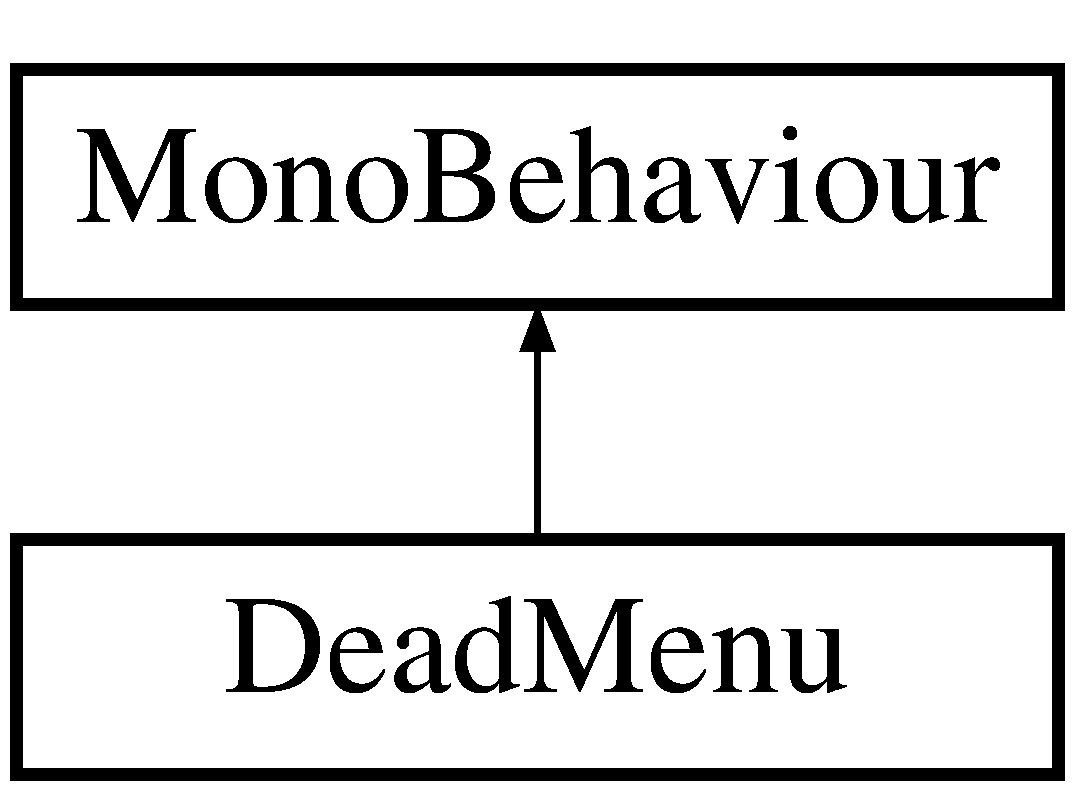
\includegraphics[height=2.000000cm]{class_dead_menu}
\end{center}
\end{figure}
\subsection*{Public Member Functions}
\begin{DoxyCompactItemize}
\item 
void \hyperlink{class_dead_menu_a26ba3bf8f5b33b3f7116f66cbc027757}{restart\+Game} ()
\begin{DoxyCompactList}\small\item\em method ini akan ditampilkan pada saat \hyperlink{class_dead_menu}{Dead\+Menu} di\+Set menjadi Active akan di tampilkan dalam bentuk button dan akan memanggil method reset dari \hyperlink{class_dead_and_restart}{Dead\+And\+Restart} class \end{DoxyCompactList}\item 
void \hyperlink{class_dead_menu_ab1eb66c9f9af09ca199d9878509fd5ba}{quit\+To\+Main} ()
\begin{DoxyCompactList}\small\item\em method ini akan ditampilkan pada saat \hyperlink{class_dead_menu}{Dead\+Menu} di\+Set menjadi Active akan di tampilkan dalam bentuk button dan akan kembali ke menu utama \end{DoxyCompactList}\end{DoxyCompactItemize}
\subsection*{Public Attributes}
\begin{DoxyCompactItemize}
\item 
\hypertarget{class_dead_menu_a264e2731503d6108fc4b88ed3f89791e}{}\label{class_dead_menu_a264e2731503d6108fc4b88ed3f89791e} 
string {\bfseries main\+Menu}
\end{DoxyCompactItemize}


\subsection{Member Function Documentation}
\hypertarget{class_dead_menu_ab1eb66c9f9af09ca199d9878509fd5ba}{}\label{class_dead_menu_ab1eb66c9f9af09ca199d9878509fd5ba} 
\index{Dead\+Menu@{Dead\+Menu}!quit\+To\+Main@{quit\+To\+Main}}
\index{quit\+To\+Main@{quit\+To\+Main}!Dead\+Menu@{Dead\+Menu}}
\subsubsection{\texorpdfstring{quit\+To\+Main()}{quitToMain()}}
{\footnotesize\ttfamily void Dead\+Menu.\+quit\+To\+Main (\begin{DoxyParamCaption}{ }\end{DoxyParamCaption})}



method ini akan ditampilkan pada saat \hyperlink{class_dead_menu}{Dead\+Menu} di\+Set menjadi Active akan di tampilkan dalam bentuk button dan akan kembali ke menu utama 

\hypertarget{class_dead_menu_a26ba3bf8f5b33b3f7116f66cbc027757}{}\label{class_dead_menu_a26ba3bf8f5b33b3f7116f66cbc027757} 
\index{Dead\+Menu@{Dead\+Menu}!restart\+Game@{restart\+Game}}
\index{restart\+Game@{restart\+Game}!Dead\+Menu@{Dead\+Menu}}
\subsubsection{\texorpdfstring{restart\+Game()}{restartGame()}}
{\footnotesize\ttfamily void Dead\+Menu.\+restart\+Game (\begin{DoxyParamCaption}{ }\end{DoxyParamCaption})}



method ini akan ditampilkan pada saat \hyperlink{class_dead_menu}{Dead\+Menu} di\+Set menjadi Active akan di tampilkan dalam bentuk button dan akan memanggil method reset dari \hyperlink{class_dead_and_restart}{Dead\+And\+Restart} class 



The documentation for this class was generated from the following file\+:\begin{DoxyCompactItemize}
\item 
C\+:/\+Users/\+Irvan/\+Documents/\+Git\+Hub/\+Tugas\+Akhir\+A\+D\+B\+O/game fix/\+Endless\+Runner/\+Assets/\+Script/Dead\+Menu.\+cs\end{DoxyCompactItemize}

\hypertarget{class_destroyer}{}\section{Destroyer Class Reference}
\label{class_destroyer}\index{Destroyer@{Destroyer}}
Inheritance diagram for Destroyer\+:\begin{figure}[H]
\begin{center}
\leavevmode
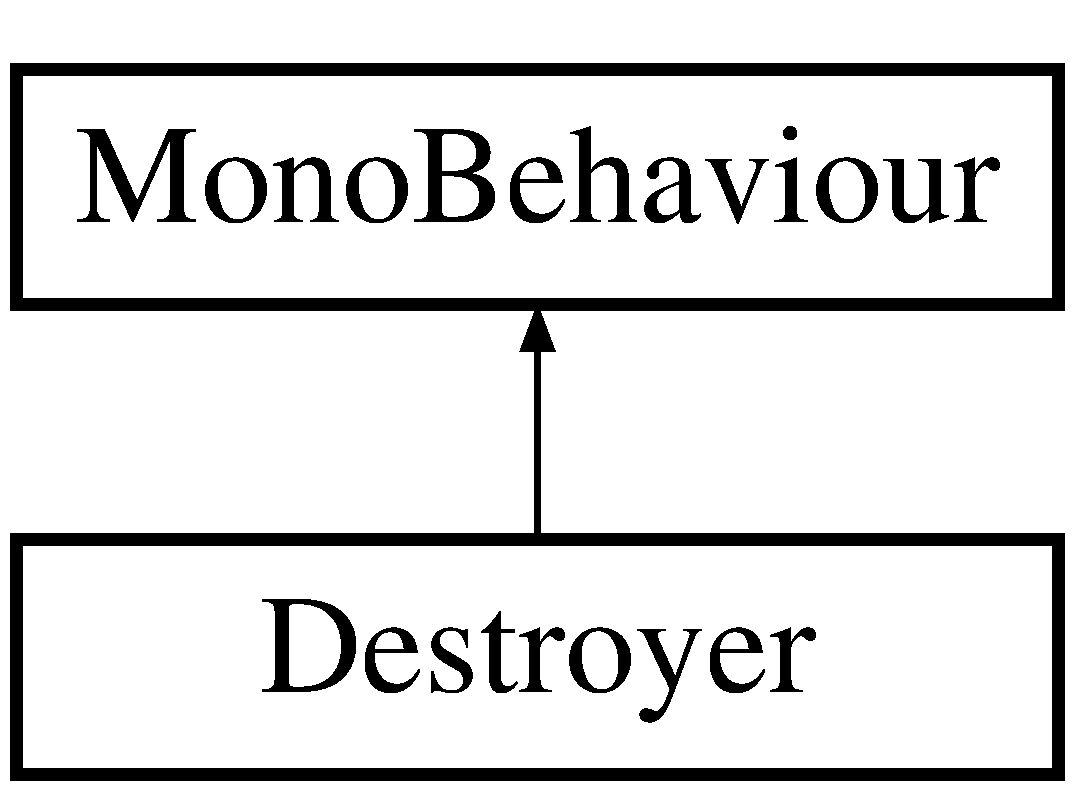
\includegraphics[height=2.000000cm]{class_destroyer}
\end{center}
\end{figure}
\subsection*{Public Attributes}
\begin{DoxyCompactItemize}
\item 
\hypertarget{class_destroyer_a029b37862396b697d50670319f4a71b9}{}\label{class_destroyer_a029b37862396b697d50670319f4a71b9} 
Game\+Object {\bfseries platform\+Destroy}
\end{DoxyCompactItemize}
\subsection*{Private Member Functions}
\begin{DoxyCompactItemize}
\item 
void \hyperlink{class_destroyer_ae187981d5587502e1e26fe5f0d5bff25}{Start} ()
\begin{DoxyCompactList}\small\item\em method akan mencari Destroky\+Point, jika ditemukan maka method akan menghancurkan game\+Object pada Destroy\+Point \end{DoxyCompactList}\item 
void \hyperlink{class_destroyer_a50232aedbebf94ee992ccb30d891bf64}{Update} ()
\begin{DoxyCompactList}\small\item\em method ini sebagai syarat,jika dipenuhi maka akan menghancurkan game\+Object \end{DoxyCompactList}\end{DoxyCompactItemize}


\subsection{Member Function Documentation}
\hypertarget{class_destroyer_ae187981d5587502e1e26fe5f0d5bff25}{}\label{class_destroyer_ae187981d5587502e1e26fe5f0d5bff25} 
\index{Destroyer@{Destroyer}!Start@{Start}}
\index{Start@{Start}!Destroyer@{Destroyer}}
\subsubsection{\texorpdfstring{Start()}{Start()}}
{\footnotesize\ttfamily void Destroyer.\+Start (\begin{DoxyParamCaption}{ }\end{DoxyParamCaption})\hspace{0.3cm}{\ttfamily [private]}}



method akan mencari Destroky\+Point, jika ditemukan maka method akan menghancurkan game\+Object pada Destroy\+Point 

\hypertarget{class_destroyer_a50232aedbebf94ee992ccb30d891bf64}{}\label{class_destroyer_a50232aedbebf94ee992ccb30d891bf64} 
\index{Destroyer@{Destroyer}!Update@{Update}}
\index{Update@{Update}!Destroyer@{Destroyer}}
\subsubsection{\texorpdfstring{Update()}{Update()}}
{\footnotesize\ttfamily void Destroyer.\+Update (\begin{DoxyParamCaption}{ }\end{DoxyParamCaption})\hspace{0.3cm}{\ttfamily [private]}}



method ini sebagai syarat,jika dipenuhi maka akan menghancurkan game\+Object 



The documentation for this class was generated from the following file\+:\begin{DoxyCompactItemize}
\item 
C\+:/\+Users/\+Irvan/\+Documents/\+Git\+Hub/\+Tugas\+Akhir\+A\+D\+B\+O/game fix/\+Endless\+Runner/\+Assets/\+Script/Destroyer.\+cs\end{DoxyCompactItemize}

\hypertarget{class_main_menu}{}\section{Main\+Menu Class Reference}
\label{class_main_menu}\index{Main\+Menu@{Main\+Menu}}
Inheritance diagram for Main\+Menu\+:\begin{figure}[H]
\begin{center}
\leavevmode
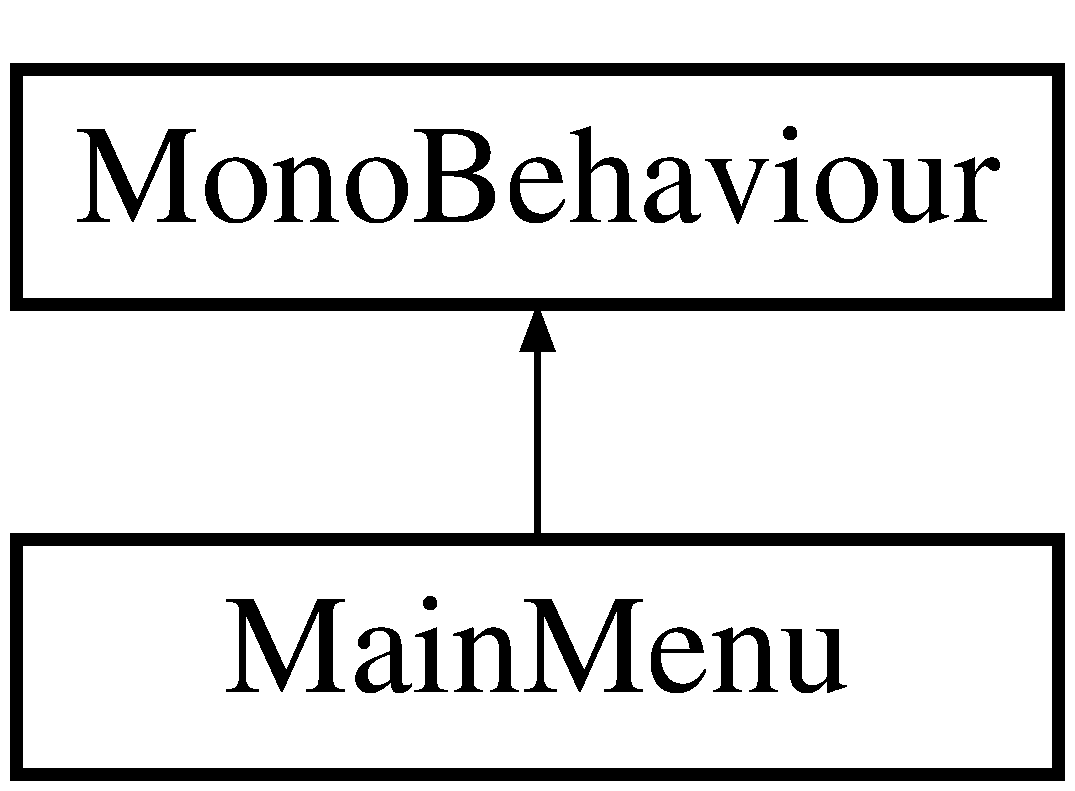
\includegraphics[height=2.000000cm]{class_main_menu}
\end{center}
\end{figure}
\subsection*{Public Member Functions}
\begin{DoxyCompactItemize}
\item 
void \hyperlink{class_main_menu_a3b485623041665dfe78d13a5b79896aa}{play} ()
\begin{DoxyCompactList}\small\item\em method play jika dijalankan akan memasukki permainan dan mulai bermain \end{DoxyCompactList}\item 
void \hyperlink{class_main_menu_ad60c51b0265c457357538cb3a6880918}{quit} ()
\begin{DoxyCompactList}\small\item\em method quit digunakan jika kita sudah ingin berhenti bermain dan menutup aplikasi \end{DoxyCompactList}\end{DoxyCompactItemize}
\subsection*{Public Attributes}
\begin{DoxyCompactItemize}
\item 
\hypertarget{class_main_menu_a935dd57ea066d80c717648224bae468d}{}\label{class_main_menu_a935dd57ea066d80c717648224bae468d} 
string {\bfseries play\+Scene}
\end{DoxyCompactItemize}


\subsection{Member Function Documentation}
\hypertarget{class_main_menu_a3b485623041665dfe78d13a5b79896aa}{}\label{class_main_menu_a3b485623041665dfe78d13a5b79896aa} 
\index{Main\+Menu@{Main\+Menu}!play@{play}}
\index{play@{play}!Main\+Menu@{Main\+Menu}}
\subsubsection{\texorpdfstring{play()}{play()}}
{\footnotesize\ttfamily void Main\+Menu.\+play (\begin{DoxyParamCaption}{ }\end{DoxyParamCaption})}



method play jika dijalankan akan memasukki permainan dan mulai bermain 

\hypertarget{class_main_menu_ad60c51b0265c457357538cb3a6880918}{}\label{class_main_menu_ad60c51b0265c457357538cb3a6880918} 
\index{Main\+Menu@{Main\+Menu}!quit@{quit}}
\index{quit@{quit}!Main\+Menu@{Main\+Menu}}
\subsubsection{\texorpdfstring{quit()}{quit()}}
{\footnotesize\ttfamily void Main\+Menu.\+quit (\begin{DoxyParamCaption}{ }\end{DoxyParamCaption})}



method quit digunakan jika kita sudah ingin berhenti bermain dan menutup aplikasi 



The documentation for this class was generated from the following file\+:\begin{DoxyCompactItemize}
\item 
C\+:/\+Users/\+Irvan/\+Documents/\+Git\+Hub/\+Tugas\+Akhir\+A\+D\+B\+O/game fix/\+Endless\+Runner/\+Assets/\+Script/Main\+Menu.\+cs\end{DoxyCompactItemize}

\hypertarget{interface_object_destroyer}{}\section{Object\+Destroyer Interface Reference}
\label{interface_object_destroyer}\index{Object\+Destroyer@{Object\+Destroyer}}
\subsection*{Public Member Functions}
\begin{DoxyCompactItemize}
\item 
\hypertarget{interface_object_destroyer_a9d672c8702f777f3246142f28468b880}{}\label{interface_object_destroyer_a9d672c8702f777f3246142f28468b880} 
void {\bfseries destroy\+Object} ()
\end{DoxyCompactItemize}


The documentation for this interface was generated from the following file\+:\begin{DoxyCompactItemize}
\item 
C\+:/\+Users/\+Irvan/\+Documents/\+Git\+Hub/\+Tugas\+Akhir\+A\+D\+B\+O/game fix/\+Endless\+Runner/\+Assets/\+Script/Object\+Destroyer.\+cs\end{DoxyCompactItemize}

\hypertarget{class_obstacle}{}\section{Obstacle Class Reference}
\label{class_obstacle}\index{Obstacle@{Obstacle}}
Inheritance diagram for Obstacle\+:\begin{figure}[H]
\begin{center}
\leavevmode
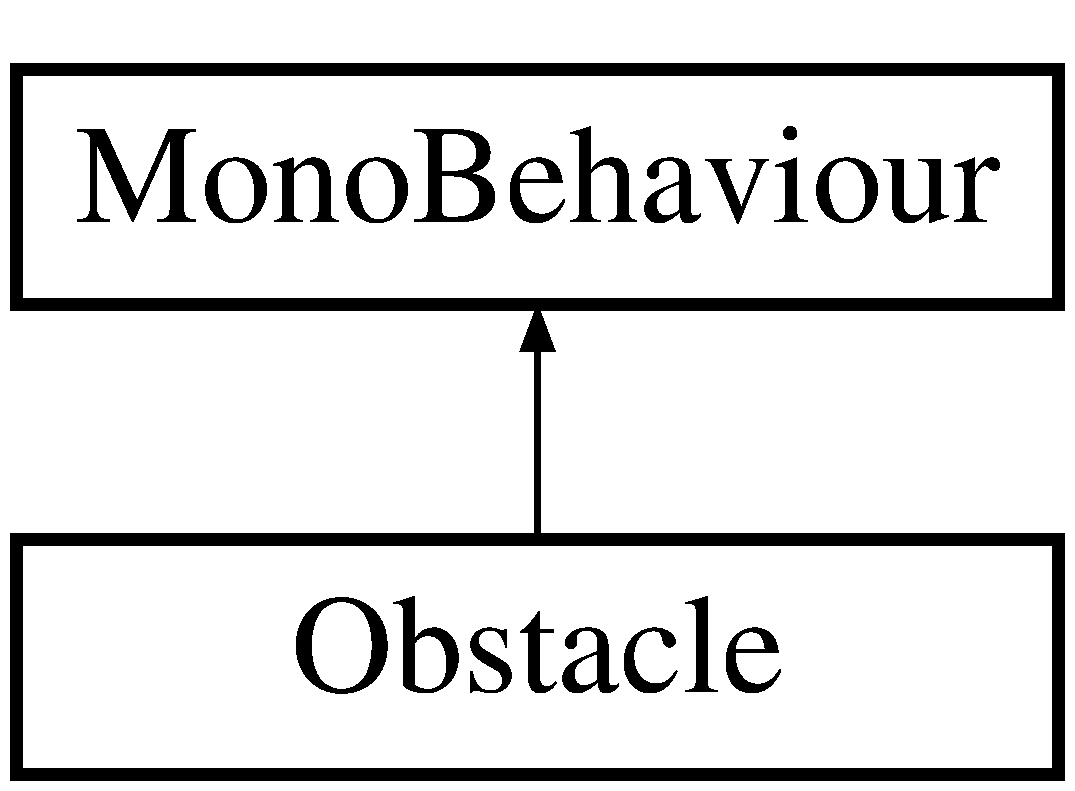
\includegraphics[height=2.000000cm]{class_obstacle}
\end{center}
\end{figure}
\subsection*{Private Member Functions}
\begin{DoxyCompactItemize}
\item 
\hypertarget{class_obstacle_adf2ba97f98b9caacbfb72675371462b0}{}\label{class_obstacle_adf2ba97f98b9caacbfb72675371462b0} 
void {\bfseries Start} ()
\item 
void \hyperlink{class_obstacle_ae0ab8556d9d584f572f1f20de2ba2890}{On\+Collision\+Enter2D} (Collision2D other)
\begin{DoxyCompactList}\small\item\em method ini dipanggil jika kedua collider(player dan obstacle) bertemu dan is\+Trigger dalam keadaan false akan memindahkan kita ke layar dead menu \end{DoxyCompactList}\end{DoxyCompactItemize}
\subsection*{Private Attributes}
\begin{DoxyCompactItemize}
\item 
\hypertarget{class_obstacle_a7c34306ff45610bfbac6aab123841c21}{}\label{class_obstacle_a7c34306ff45610bfbac6aab123841c21} 
\hyperlink{class_dead_and_restart}{Dead\+And\+Restart} {\bfseries dead\+And\+Restart}
\end{DoxyCompactItemize}


\subsection{Member Function Documentation}
\hypertarget{class_obstacle_ae0ab8556d9d584f572f1f20de2ba2890}{}\label{class_obstacle_ae0ab8556d9d584f572f1f20de2ba2890} 
\index{Obstacle@{Obstacle}!On\+Collision\+Enter2D@{On\+Collision\+Enter2D}}
\index{On\+Collision\+Enter2D@{On\+Collision\+Enter2D}!Obstacle@{Obstacle}}
\subsubsection{\texorpdfstring{On\+Collision\+Enter2\+D()}{OnCollisionEnter2D()}}
{\footnotesize\ttfamily void Obstacle.\+On\+Collision\+Enter2D (\begin{DoxyParamCaption}\item[{Collision2D}]{other }\end{DoxyParamCaption})\hspace{0.3cm}{\ttfamily [private]}}



method ini dipanggil jika kedua collider(player dan obstacle) bertemu dan is\+Trigger dalam keadaan false akan memindahkan kita ke layar dead menu 


\begin{DoxyParams}{Parameters}
{\em other} & Other.\\
\hline
\end{DoxyParams}


The documentation for this class was generated from the following file\+:\begin{DoxyCompactItemize}
\item 
C\+:/\+Users/\+Irvan/\+Documents/\+Git\+Hub/\+Tugas\+Akhir\+A\+D\+B\+O/game fix/\+Endless\+Runner/\+Assets/\+Script/Obstacle.\+cs\end{DoxyCompactItemize}

\hypertarget{class_obstacle_controller}{}\section{Obstacle\+Controller Class Reference}
\label{class_obstacle_controller}\index{Obstacle\+Controller@{Obstacle\+Controller}}
Inheritance diagram for Obstacle\+Controller\+:\begin{figure}[H]
\begin{center}
\leavevmode
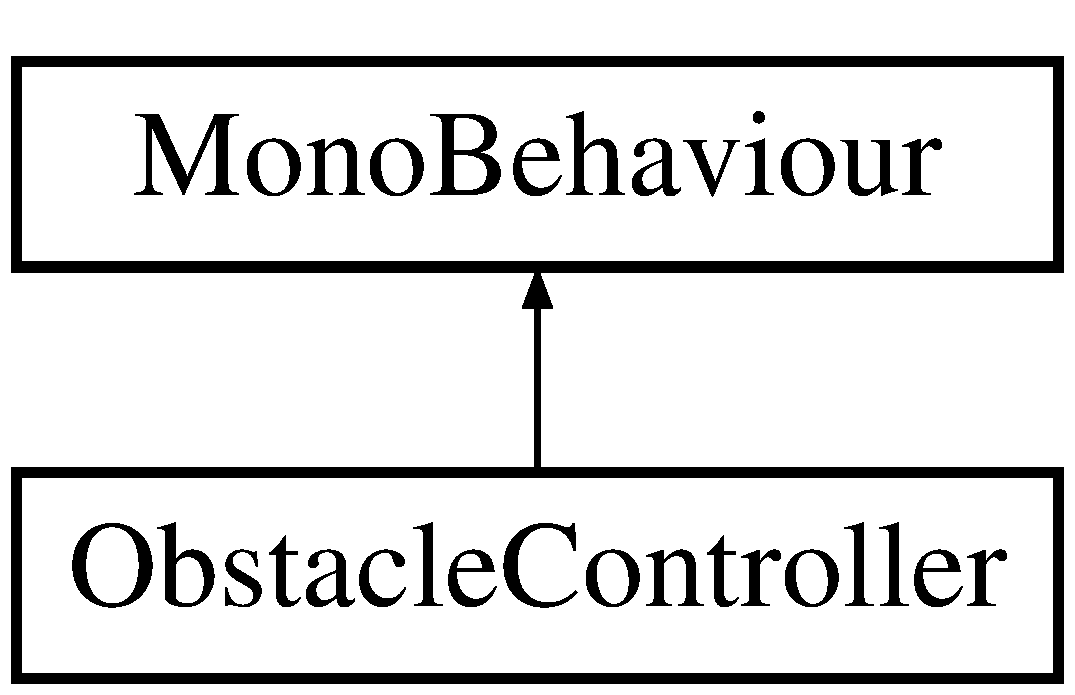
\includegraphics[height=2.000000cm]{class_obstacle_controller}
\end{center}
\end{figure}
\subsection*{Public Member Functions}
\begin{DoxyCompactItemize}
\item 
\hypertarget{class_obstacle_controller_a4c3be71b2f4cc9228123fbe62cf090de}{}\label{class_obstacle_controller_a4c3be71b2f4cc9228123fbe62cf090de} 
void {\bfseries re\+Start} ()
\end{DoxyCompactItemize}
\subsection*{Private Member Functions}
\begin{DoxyCompactItemize}
\item 
\hypertarget{class_obstacle_controller_a5bc9c314bdf442520b7d8499f8b57849}{}\label{class_obstacle_controller_a5bc9c314bdf442520b7d8499f8b57849} 
void {\bfseries Start} ()
\item 
void \hyperlink{class_obstacle_controller_a2d1939f5e5a56507a9b0cdcfe70b38f9}{On\+Trigger\+Enter2D} (Collider2D other)
\begin{DoxyCompactList}\small\item\em method ini akan dipanggil jika karakter menyentuh collider maka akan memanggil method Create\+Obstacle \end{DoxyCompactList}\item 
void \hyperlink{class_obstacle_controller_ac4ade82f15fed22429690b7f20aee930}{Create\+Obstacle} ()
\begin{DoxyCompactList}\small\item\em method ini akan membuat sebuah obstacle baru (babi/api) tergantung pada nilai i \end{DoxyCompactList}\end{DoxyCompactItemize}
\subsection*{Private Attributes}
\begin{DoxyCompactItemize}
\item 
\hypertarget{class_obstacle_controller_a2f1cb4b6681d630286032d9ad3446342}{}\label{class_obstacle_controller_a2f1cb4b6681d630286032d9ad3446342} 
Game\+Object \mbox{[}$\,$\mbox{]} {\bfseries obstacle} = new Game\+Object\mbox{[}2\mbox{]}
\item 
\hypertarget{class_obstacle_controller_acec4d4decf5a2e54b41db74c15378396}{}\label{class_obstacle_controller_acec4d4decf5a2e54b41db74c15378396} 
int {\bfseries i}
\item 
\hypertarget{class_obstacle_controller_a80abe8f0b50a4dbede423349a1cc4a3a}{}\label{class_obstacle_controller_a80abe8f0b50a4dbede423349a1cc4a3a} 
Vector2 {\bfseries pos\+Now}
\item 
\hypertarget{class_obstacle_controller_a8cbe87dc8debfacb1afe0b41d0881c3e}{}\label{class_obstacle_controller_a8cbe87dc8debfacb1afe0b41d0881c3e} 
Vector2 {\bfseries pos\+Now\+Babi}
\end{DoxyCompactItemize}


\subsection{Member Function Documentation}
\hypertarget{class_obstacle_controller_ac4ade82f15fed22429690b7f20aee930}{}\label{class_obstacle_controller_ac4ade82f15fed22429690b7f20aee930} 
\index{Obstacle\+Controller@{Obstacle\+Controller}!Create\+Obstacle@{Create\+Obstacle}}
\index{Create\+Obstacle@{Create\+Obstacle}!Obstacle\+Controller@{Obstacle\+Controller}}
\subsubsection{\texorpdfstring{Create\+Obstacle()}{CreateObstacle()}}
{\footnotesize\ttfamily void Obstacle\+Controller.\+Create\+Obstacle (\begin{DoxyParamCaption}{ }\end{DoxyParamCaption})\hspace{0.3cm}{\ttfamily [private]}}



method ini akan membuat sebuah obstacle baru (babi/api) tergantung pada nilai i 

\hypertarget{class_obstacle_controller_a2d1939f5e5a56507a9b0cdcfe70b38f9}{}\label{class_obstacle_controller_a2d1939f5e5a56507a9b0cdcfe70b38f9} 
\index{Obstacle\+Controller@{Obstacle\+Controller}!On\+Trigger\+Enter2D@{On\+Trigger\+Enter2D}}
\index{On\+Trigger\+Enter2D@{On\+Trigger\+Enter2D}!Obstacle\+Controller@{Obstacle\+Controller}}
\subsubsection{\texorpdfstring{On\+Trigger\+Enter2\+D()}{OnTriggerEnter2D()}}
{\footnotesize\ttfamily void Obstacle\+Controller.\+On\+Trigger\+Enter2D (\begin{DoxyParamCaption}\item[{Collider2D}]{other }\end{DoxyParamCaption})\hspace{0.3cm}{\ttfamily [private]}}



method ini akan dipanggil jika karakter menyentuh collider maka akan memanggil method Create\+Obstacle 


\begin{DoxyParams}{Parameters}
{\em other} & Other.\\
\hline
\end{DoxyParams}


The documentation for this class was generated from the following file\+:\begin{DoxyCompactItemize}
\item 
C\+:/\+Users/\+Irvan/\+Documents/\+Git\+Hub/\+Tugas\+Akhir\+A\+D\+B\+O/game fix/\+Endless\+Runner/\+Assets/\+Script/Obstacle\+Controller.\+cs\end{DoxyCompactItemize}

\hypertarget{class_pause_menu}{}\section{Pause\+Menu Class Reference}
\label{class_pause_menu}\index{Pause\+Menu@{Pause\+Menu}}
Inheritance diagram for Pause\+Menu\+:\begin{figure}[H]
\begin{center}
\leavevmode
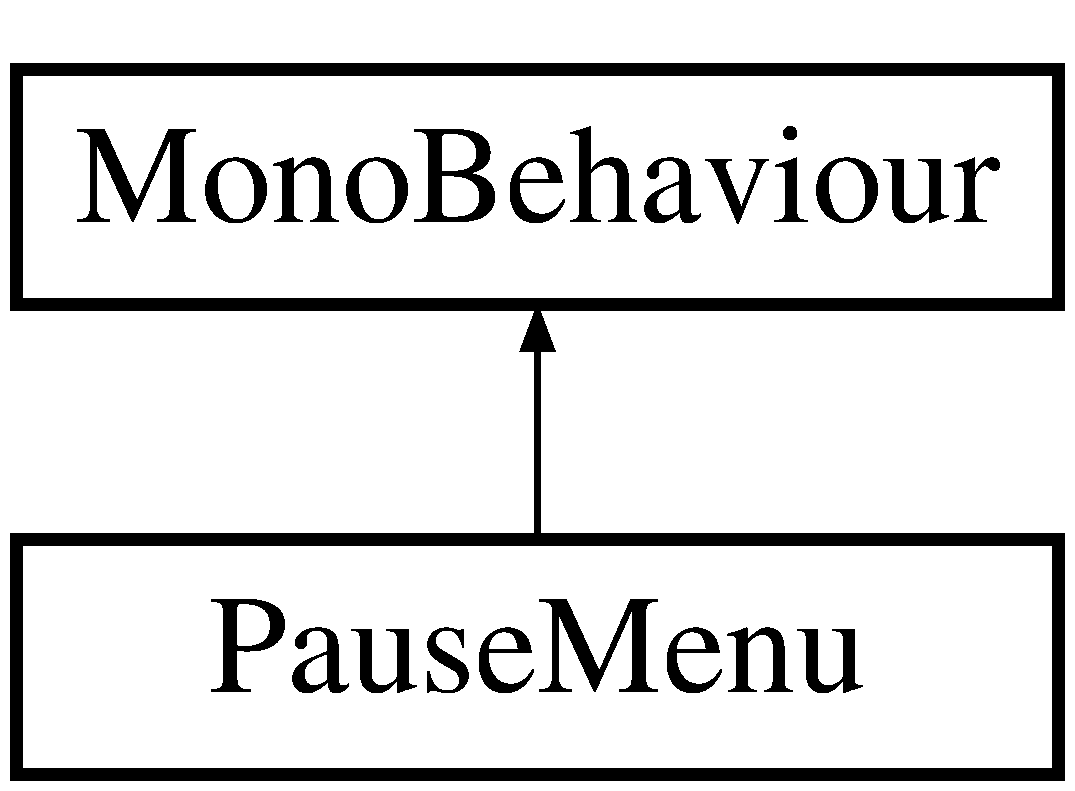
\includegraphics[height=2.000000cm]{class_pause_menu}
\end{center}
\end{figure}
\subsection*{Public Member Functions}
\begin{DoxyCompactItemize}
\item 
\hypertarget{class_pause_menu_af497942ddf1f2b7eb11c054c865353ec}{}\label{class_pause_menu_af497942ddf1f2b7eb11c054c865353ec} 
void {\bfseries pause\+Game} ()
\item 
\hypertarget{class_pause_menu_a8eea4a2ea1b10e58d6b376899a2966d3}{}\label{class_pause_menu_a8eea4a2ea1b10e58d6b376899a2966d3} 
void {\bfseries resume\+Game} ()
\item 
void \hyperlink{class_pause_menu_ac64b5f82050f56e6553e7b60e926c1ed}{restart\+Game} ()
\begin{DoxyCompactList}\small\item\em method ini akan ditampilkan pada saat \hyperlink{class_dead_menu}{Dead\+Menu} di\+Set menjadi Active akan di tampilkan dalam bentuk button dan akan memanggil method reset dari \hyperlink{class_dead_and_restart}{Dead\+And\+Restart} class \end{DoxyCompactList}\item 
void \hyperlink{class_pause_menu_abd6872204e8867b9823bce94cbb36b54}{quit\+To\+Main} ()
\begin{DoxyCompactList}\small\item\em method ini akan ditampilkan pada saat \hyperlink{class_dead_menu}{Dead\+Menu} di\+Set menjadi Active akan di tampilkan dalam bentuk button dan akan kembali ke menu utama \end{DoxyCompactList}\end{DoxyCompactItemize}
\subsection*{Public Attributes}
\begin{DoxyCompactItemize}
\item 
\hypertarget{class_pause_menu_ab66fa055eeaf9ed2236f89d7192e9d84}{}\label{class_pause_menu_ab66fa055eeaf9ed2236f89d7192e9d84} 
string {\bfseries main\+Menu}
\item 
\hypertarget{class_pause_menu_a2a4732fd962c6aa136a867be16b71cc2}{}\label{class_pause_menu_a2a4732fd962c6aa136a867be16b71cc2} 
Game\+Object {\bfseries pause\+Menu}
\end{DoxyCompactItemize}


\subsection{Member Function Documentation}
\hypertarget{class_pause_menu_abd6872204e8867b9823bce94cbb36b54}{}\label{class_pause_menu_abd6872204e8867b9823bce94cbb36b54} 
\index{Pause\+Menu@{Pause\+Menu}!quit\+To\+Main@{quit\+To\+Main}}
\index{quit\+To\+Main@{quit\+To\+Main}!Pause\+Menu@{Pause\+Menu}}
\subsubsection{\texorpdfstring{quit\+To\+Main()}{quitToMain()}}
{\footnotesize\ttfamily void Pause\+Menu.\+quit\+To\+Main (\begin{DoxyParamCaption}{ }\end{DoxyParamCaption})}



method ini akan ditampilkan pada saat \hyperlink{class_dead_menu}{Dead\+Menu} di\+Set menjadi Active akan di tampilkan dalam bentuk button dan akan kembali ke menu utama 

\hypertarget{class_pause_menu_ac64b5f82050f56e6553e7b60e926c1ed}{}\label{class_pause_menu_ac64b5f82050f56e6553e7b60e926c1ed} 
\index{Pause\+Menu@{Pause\+Menu}!restart\+Game@{restart\+Game}}
\index{restart\+Game@{restart\+Game}!Pause\+Menu@{Pause\+Menu}}
\subsubsection{\texorpdfstring{restart\+Game()}{restartGame()}}
{\footnotesize\ttfamily void Pause\+Menu.\+restart\+Game (\begin{DoxyParamCaption}{ }\end{DoxyParamCaption})}



method ini akan ditampilkan pada saat \hyperlink{class_dead_menu}{Dead\+Menu} di\+Set menjadi Active akan di tampilkan dalam bentuk button dan akan memanggil method reset dari \hyperlink{class_dead_and_restart}{Dead\+And\+Restart} class 



The documentation for this class was generated from the following file\+:\begin{DoxyCompactItemize}
\item 
C\+:/\+Users/\+Irvan/\+Documents/\+Git\+Hub/\+Tugas\+Akhir\+A\+D\+B\+O/game fix/\+Endless\+Runner/\+Assets/\+Script/Pause\+Menu.\+cs\end{DoxyCompactItemize}

\hypertarget{class_platform_generator}{}\section{Platform\+Generator Class Reference}
\label{class_platform_generator}\index{Platform\+Generator@{Platform\+Generator}}
Inheritance diagram for Platform\+Generator\+:\begin{figure}[H]
\begin{center}
\leavevmode
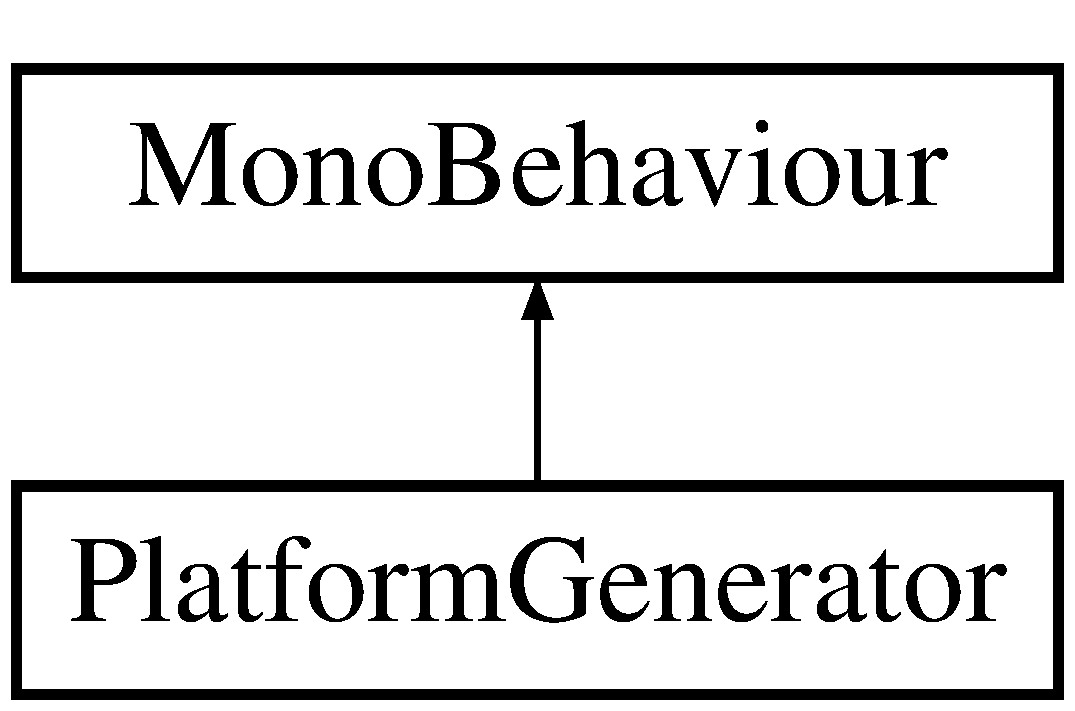
\includegraphics[height=2.000000cm]{class_platform_generator}
\end{center}
\end{figure}
\subsection*{Public Attributes}
\begin{DoxyCompactItemize}
\item 
\hypertarget{class_platform_generator_aa8fe8501862e7e300c00d59e57586a47}{}\label{class_platform_generator_aa8fe8501862e7e300c00d59e57586a47} 
Game\+Object {\bfseries the\+Platform}
\item 
\hypertarget{class_platform_generator_aad78bda099715573856e053b41a355fc}{}\label{class_platform_generator_aad78bda099715573856e053b41a355fc} 
Transform {\bfseries generation\+Point}
\end{DoxyCompactItemize}
\subsection*{Private Member Functions}
\begin{DoxyCompactItemize}
\item 
void \hyperlink{class_platform_generator_a4a9f8f525415c599d761c8371734619d}{Start} ()
\begin{DoxyCompactList}\small\item\em method ini seperti constructor untuk menentukan collider platform dan posisinya. \end{DoxyCompactList}\item 
void \hyperlink{class_platform_generator_a8e50d153f28945c3755b9d9bfb2fde9a}{Update} ()
\begin{DoxyCompactList}\small\item\em method ini akan memanggil method generate jika sudah memenuhi syarat generation\+Point \end{DoxyCompactList}\item 
void \hyperlink{class_platform_generator_aa6c531bd8acd0de80999c4033e4f0a8e}{generate} ()
\begin{DoxyCompactList}\small\item\em method ini digunakan untuk menambah platform/meng-\/kloning platform secara terus-\/menerus \end{DoxyCompactList}\end{DoxyCompactItemize}
\subsection*{Private Attributes}
\begin{DoxyCompactItemize}
\item 
\hypertarget{class_platform_generator_abad4d150ee047d135102b79663d718ec}{}\label{class_platform_generator_abad4d150ee047d135102b79663d718ec} 
float {\bfseries platform\+Width}
\end{DoxyCompactItemize}


\subsection{Member Function Documentation}
\hypertarget{class_platform_generator_aa6c531bd8acd0de80999c4033e4f0a8e}{}\label{class_platform_generator_aa6c531bd8acd0de80999c4033e4f0a8e} 
\index{Platform\+Generator@{Platform\+Generator}!generate@{generate}}
\index{generate@{generate}!Platform\+Generator@{Platform\+Generator}}
\subsubsection{\texorpdfstring{generate()}{generate()}}
{\footnotesize\ttfamily void Platform\+Generator.\+generate (\begin{DoxyParamCaption}{ }\end{DoxyParamCaption})\hspace{0.3cm}{\ttfamily [private]}}



method ini digunakan untuk menambah platform/meng-\/kloning platform secara terus-\/menerus 

\hypertarget{class_platform_generator_a4a9f8f525415c599d761c8371734619d}{}\label{class_platform_generator_a4a9f8f525415c599d761c8371734619d} 
\index{Platform\+Generator@{Platform\+Generator}!Start@{Start}}
\index{Start@{Start}!Platform\+Generator@{Platform\+Generator}}
\subsubsection{\texorpdfstring{Start()}{Start()}}
{\footnotesize\ttfamily void Platform\+Generator.\+Start (\begin{DoxyParamCaption}{ }\end{DoxyParamCaption})\hspace{0.3cm}{\ttfamily [private]}}



method ini seperti constructor untuk menentukan collider platform dan posisinya. 

\hypertarget{class_platform_generator_a8e50d153f28945c3755b9d9bfb2fde9a}{}\label{class_platform_generator_a8e50d153f28945c3755b9d9bfb2fde9a} 
\index{Platform\+Generator@{Platform\+Generator}!Update@{Update}}
\index{Update@{Update}!Platform\+Generator@{Platform\+Generator}}
\subsubsection{\texorpdfstring{Update()}{Update()}}
{\footnotesize\ttfamily void Platform\+Generator.\+Update (\begin{DoxyParamCaption}{ }\end{DoxyParamCaption})\hspace{0.3cm}{\ttfamily [private]}}



method ini akan memanggil method generate jika sudah memenuhi syarat generation\+Point 



The documentation for this class was generated from the following file\+:\begin{DoxyCompactItemize}
\item 
C\+:/\+Users/\+Irvan/\+Documents/\+Git\+Hub/\+Tugas\+Akhir\+A\+D\+B\+O/game fix/\+Endless\+Runner/\+Assets/\+Script/Platform\+Generator.\+cs\end{DoxyCompactItemize}

\hypertarget{class_player_controller}{}\section{Player\+Controller Class Reference}
\label{class_player_controller}\index{Player\+Controller@{Player\+Controller}}
Inheritance diagram for Player\+Controller\+:\begin{figure}[H]
\begin{center}
\leavevmode
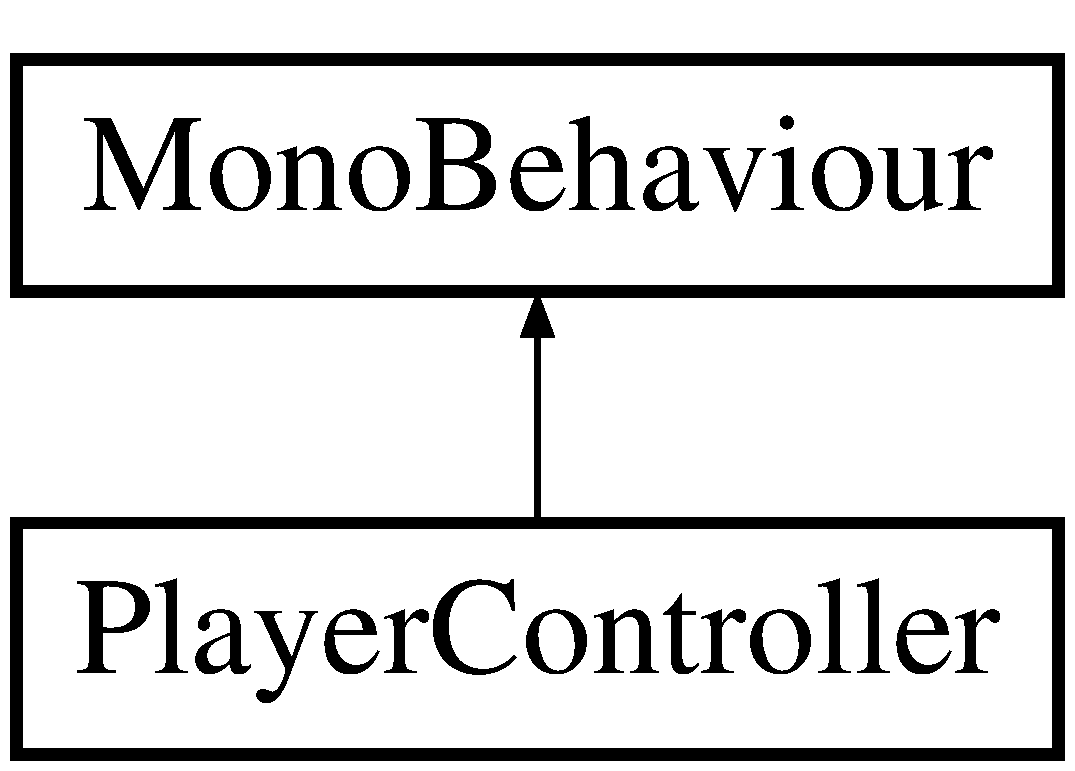
\includegraphics[height=2.000000cm]{class_player_controller}
\end{center}
\end{figure}
\subsection*{Public Member Functions}
\begin{DoxyCompactItemize}
\item 
void \hyperlink{class_player_controller_adb52e7f8ab39c74e1922393d5015a70a}{set\+To\+Start} ()
\begin{DoxyCompactList}\small\item\em method ini bekerja seperti method start , tetapi digunakan saat merestart game dalam dead menu \end{DoxyCompactList}\end{DoxyCompactItemize}
\subsection*{Public Attributes}
\begin{DoxyCompactItemize}
\item 
\hypertarget{class_player_controller_a7c109871eba0057fd2aa1856522a346d}{}\label{class_player_controller_a7c109871eba0057fd2aa1856522a346d} 
float {\bfseries jump\+Force}
\item 
\hypertarget{class_player_controller_a365831d3d6fc1d27a30086ad467305a1}{}\label{class_player_controller_a365831d3d6fc1d27a30086ad467305a1} 
float {\bfseries jump\+Hold\+Time}
\item 
\hypertarget{class_player_controller_abb12e85ca1b12efdbc8684bff2e19c4c}{}\label{class_player_controller_abb12e85ca1b12efdbc8684bff2e19c4c} 
float {\bfseries move\+Speed}
\item 
\hypertarget{class_player_controller_a15aeb9e2671ba8dc7124be81397f84be}{}\label{class_player_controller_a15aeb9e2671ba8dc7124be81397f84be} 
float {\bfseries speed\+Multiplier}
\item 
\hypertarget{class_player_controller_a23820dab3461bec7fe783e801c27c8ff}{}\label{class_player_controller_a23820dab3461bec7fe783e801c27c8ff} 
float {\bfseries jarak\+Tempuh}
\item 
\hypertarget{class_player_controller_a1810294c934464cd555eec1107d2379b}{}\label{class_player_controller_a1810294c934464cd555eec1107d2379b} 
bool {\bfseries grounded}
\item 
\hypertarget{class_player_controller_a63d4bd8d38ba41b7aa45833104c11813}{}\label{class_player_controller_a63d4bd8d38ba41b7aa45833104c11813} 
bool {\bfseries slide}
\item 
\hypertarget{class_player_controller_a5280def315a8ef1d16620890a1523273}{}\label{class_player_controller_a5280def315a8ef1d16620890a1523273} 
Layer\+Mask {\bfseries what\+Is\+Ground}
\item 
\hypertarget{class_player_controller_ab1e1eba1b79ab5d5771099e67b0057fb}{}\label{class_player_controller_ab1e1eba1b79ab5d5771099e67b0057fb} 
Audio\+Source {\bfseries jump\+Sound}
\end{DoxyCompactItemize}
\subsection*{Private Member Functions}
\begin{DoxyCompactItemize}
\item 
\hypertarget{class_player_controller_ae1117d9c4da3193181cddad2c814e467}{}\label{class_player_controller_ae1117d9c4da3193181cddad2c814e467} 
void {\bfseries Start} ()
\item 
\hypertarget{class_player_controller_ae8bc83dffb99867a04be016473ed2c43}{}\label{class_player_controller_ae8bc83dffb99867a04be016473ed2c43} 
void {\bfseries Update} ()
\item 
void \hyperlink{class_player_controller_accbeb6b75b9f6067679b960a91581de6}{speed} ()
\begin{DoxyCompactList}\small\item\em mengatur kecepatan karakter \end{DoxyCompactList}\item 
void \hyperlink{class_player_controller_a413e8e34033169093b21b38bf6bd0b34}{jump} ()
\begin{DoxyCompactList}\small\item\em mengatur cara karakter melompat \end{DoxyCompactList}\item 
void \hyperlink{class_player_controller_afd5b28f0a9018e11fc879c93107c7a37}{jump\+Hold} ()
\begin{DoxyCompactList}\small\item\em mengatur lama melompat jika tombol di tahan \end{DoxyCompactList}\item 
void \hyperlink{class_player_controller_af65ea7266683911055939bfad8c4248b}{jump\+Release} ()
\begin{DoxyCompactList}\small\item\em mengatur agar tidak dapat melompat lagi jika tombol di lepas \end{DoxyCompactList}\end{DoxyCompactItemize}
\subsection*{Private Attributes}
\begin{DoxyCompactItemize}
\item 
\hypertarget{class_player_controller_a964dd786d816edf28dfb22e076e7fb6e}{}\label{class_player_controller_a964dd786d816edf28dfb22e076e7fb6e} 
float {\bfseries jump\+Hold\+Time\+Counter}
\item 
\hypertarget{class_player_controller_a1b529005d052b11fe8843e3fa6de3a2a}{}\label{class_player_controller_a1b529005d052b11fe8843e3fa6de3a2a} 
float {\bfseries nambah\+Jarak}
\item 
\hypertarget{class_player_controller_ae7c227462646c52ac0b35517303ea57d}{}\label{class_player_controller_ae7c227462646c52ac0b35517303ea57d} 
Rigidbody2D {\bfseries my\+Rigid\+Body}
\item 
\hypertarget{class_player_controller_a0e793baf5b00ac0d6bcf367060db5f55}{}\label{class_player_controller_a0e793baf5b00ac0d6bcf367060db5f55} 
Collider2D {\bfseries my\+Collider}
\item 
\hypertarget{class_player_controller_a34fe46e66072a17354236ce4c9909767}{}\label{class_player_controller_a34fe46e66072a17354236ce4c9909767} 
Animator {\bfseries my\+Animator}
\item 
\hypertarget{class_player_controller_a51abe7ff34134e22526284c8492ac2af}{}\label{class_player_controller_a51abe7ff34134e22526284c8492ac2af} 
Box\+Collider2D {\bfseries box\+Col}
\item 
\hypertarget{class_player_controller_abe1551a2d9b41ba6c7ce2895867eea18}{}\label{class_player_controller_abe1551a2d9b41ba6c7ce2895867eea18} 
Vector3 {\bfseries ukuran\+Awal}
\end{DoxyCompactItemize}


\subsection{Member Function Documentation}
\hypertarget{class_player_controller_a413e8e34033169093b21b38bf6bd0b34}{}\label{class_player_controller_a413e8e34033169093b21b38bf6bd0b34} 
\index{Player\+Controller@{Player\+Controller}!jump@{jump}}
\index{jump@{jump}!Player\+Controller@{Player\+Controller}}
\subsubsection{\texorpdfstring{jump()}{jump()}}
{\footnotesize\ttfamily void Player\+Controller.\+jump (\begin{DoxyParamCaption}{ }\end{DoxyParamCaption})\hspace{0.3cm}{\ttfamily [private]}}



mengatur cara karakter melompat 

\hypertarget{class_player_controller_afd5b28f0a9018e11fc879c93107c7a37}{}\label{class_player_controller_afd5b28f0a9018e11fc879c93107c7a37} 
\index{Player\+Controller@{Player\+Controller}!jump\+Hold@{jump\+Hold}}
\index{jump\+Hold@{jump\+Hold}!Player\+Controller@{Player\+Controller}}
\subsubsection{\texorpdfstring{jump\+Hold()}{jumpHold()}}
{\footnotesize\ttfamily void Player\+Controller.\+jump\+Hold (\begin{DoxyParamCaption}{ }\end{DoxyParamCaption})\hspace{0.3cm}{\ttfamily [private]}}



mengatur lama melompat jika tombol di tahan 

\hypertarget{class_player_controller_af65ea7266683911055939bfad8c4248b}{}\label{class_player_controller_af65ea7266683911055939bfad8c4248b} 
\index{Player\+Controller@{Player\+Controller}!jump\+Release@{jump\+Release}}
\index{jump\+Release@{jump\+Release}!Player\+Controller@{Player\+Controller}}
\subsubsection{\texorpdfstring{jump\+Release()}{jumpRelease()}}
{\footnotesize\ttfamily void Player\+Controller.\+jump\+Release (\begin{DoxyParamCaption}{ }\end{DoxyParamCaption})\hspace{0.3cm}{\ttfamily [private]}}



mengatur agar tidak dapat melompat lagi jika tombol di lepas 

\hypertarget{class_player_controller_adb52e7f8ab39c74e1922393d5015a70a}{}\label{class_player_controller_adb52e7f8ab39c74e1922393d5015a70a} 
\index{Player\+Controller@{Player\+Controller}!set\+To\+Start@{set\+To\+Start}}
\index{set\+To\+Start@{set\+To\+Start}!Player\+Controller@{Player\+Controller}}
\subsubsection{\texorpdfstring{set\+To\+Start()}{setToStart()}}
{\footnotesize\ttfamily void Player\+Controller.\+set\+To\+Start (\begin{DoxyParamCaption}{ }\end{DoxyParamCaption})}



method ini bekerja seperti method start , tetapi digunakan saat merestart game dalam dead menu 

\hypertarget{class_player_controller_accbeb6b75b9f6067679b960a91581de6}{}\label{class_player_controller_accbeb6b75b9f6067679b960a91581de6} 
\index{Player\+Controller@{Player\+Controller}!speed@{speed}}
\index{speed@{speed}!Player\+Controller@{Player\+Controller}}
\subsubsection{\texorpdfstring{speed()}{speed()}}
{\footnotesize\ttfamily void Player\+Controller.\+speed (\begin{DoxyParamCaption}{ }\end{DoxyParamCaption})\hspace{0.3cm}{\ttfamily [private]}}



mengatur kecepatan karakter 



The documentation for this class was generated from the following file\+:\begin{DoxyCompactItemize}
\item 
C\+:/\+Users/\+Irvan/\+Documents/\+Git\+Hub/\+Tugas\+Akhir\+A\+D\+B\+O/game fix/\+Endless\+Runner/\+Assets/\+Script/Player\+Controller.\+cs\end{DoxyCompactItemize}

\hypertarget{class_score_controller}{}\section{Score\+Controller Class Reference}
\label{class_score_controller}\index{Score\+Controller@{Score\+Controller}}
Inheritance diagram for Score\+Controller\+:\begin{figure}[H]
\begin{center}
\leavevmode
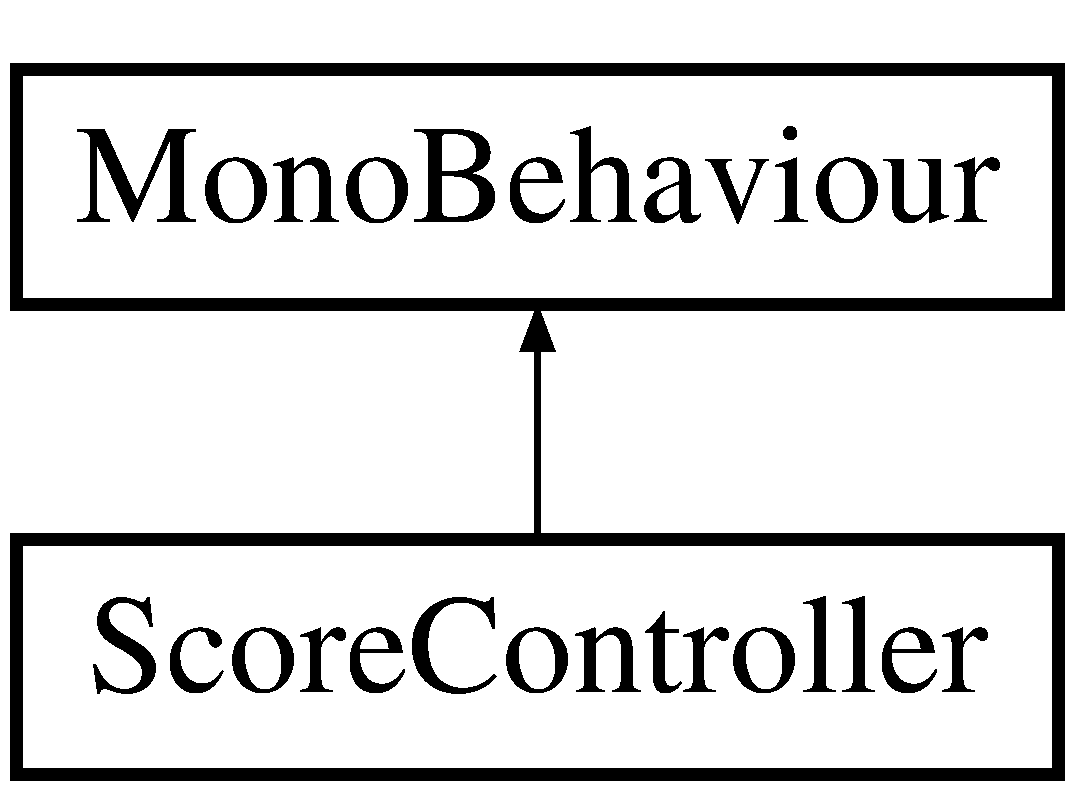
\includegraphics[height=2.000000cm]{class_score_controller}
\end{center}
\end{figure}
\subsection*{Public Attributes}
\begin{DoxyCompactItemize}
\item 
\hypertarget{class_score_controller_a1be2da4c8951c565e55406e546d48651}{}\label{class_score_controller_a1be2da4c8951c565e55406e546d48651} 
int {\bfseries score}
\item 
\hypertarget{class_score_controller_af25aeff6d92cb0bfe9d0c6bbed6b450b}{}\label{class_score_controller_af25aeff6d92cb0bfe9d0c6bbed6b450b} 
int {\bfseries high\+Score}
\item 
\hypertarget{class_score_controller_a7152e2b1715326c8a1ab07c6b3d1ca4b}{}\label{class_score_controller_a7152e2b1715326c8a1ab07c6b3d1ca4b} 
Text {\bfseries score\+Text}
\item 
\hypertarget{class_score_controller_a2ab288a8f264ce21418e90ed8f175f00}{}\label{class_score_controller_a2ab288a8f264ce21418e90ed8f175f00} 
Text {\bfseries high\+Score\+Text}
\item 
\hypertarget{class_score_controller_a396f8b7a21830617b640e67e4e9a14e7}{}\label{class_score_controller_a396f8b7a21830617b640e67e4e9a14e7} 
\hyperlink{class_player_controller}{Player\+Controller} {\bfseries player}
\end{DoxyCompactItemize}
\subsection*{Private Member Functions}
\begin{DoxyCompactItemize}
\item 
void \hyperlink{class_score_controller_a24c8b4f29b0e90a9bf721023cd1c581d}{Start} ()
\begin{DoxyCompactList}\small\item\em men-\/set score dan highscore di awal permainan \end{DoxyCompactList}\item 
void \hyperlink{class_score_controller_a30682b0eb78ea3820856810083221ee6}{Update} ()
\begin{DoxyCompactList}\small\item\em memanggil method inc\+Score \end{DoxyCompactList}\item 
void \hyperlink{class_score_controller_a9af998d59d5024890bc86f91e5ce276e}{inc\+Score} ()
\begin{DoxyCompactList}\small\item\em method ini digunakan untuk menambah skor saat bermain \end{DoxyCompactList}\end{DoxyCompactItemize}


\subsection{Member Function Documentation}
\hypertarget{class_score_controller_a9af998d59d5024890bc86f91e5ce276e}{}\label{class_score_controller_a9af998d59d5024890bc86f91e5ce276e} 
\index{Score\+Controller@{Score\+Controller}!inc\+Score@{inc\+Score}}
\index{inc\+Score@{inc\+Score}!Score\+Controller@{Score\+Controller}}
\subsubsection{\texorpdfstring{inc\+Score()}{incScore()}}
{\footnotesize\ttfamily void Score\+Controller.\+inc\+Score (\begin{DoxyParamCaption}{ }\end{DoxyParamCaption})\hspace{0.3cm}{\ttfamily [private]}}



method ini digunakan untuk menambah skor saat bermain 

\hypertarget{class_score_controller_a24c8b4f29b0e90a9bf721023cd1c581d}{}\label{class_score_controller_a24c8b4f29b0e90a9bf721023cd1c581d} 
\index{Score\+Controller@{Score\+Controller}!Start@{Start}}
\index{Start@{Start}!Score\+Controller@{Score\+Controller}}
\subsubsection{\texorpdfstring{Start()}{Start()}}
{\footnotesize\ttfamily void Score\+Controller.\+Start (\begin{DoxyParamCaption}{ }\end{DoxyParamCaption})\hspace{0.3cm}{\ttfamily [private]}}



men-\/set score dan highscore di awal permainan 

\hypertarget{class_score_controller_a30682b0eb78ea3820856810083221ee6}{}\label{class_score_controller_a30682b0eb78ea3820856810083221ee6} 
\index{Score\+Controller@{Score\+Controller}!Update@{Update}}
\index{Update@{Update}!Score\+Controller@{Score\+Controller}}
\subsubsection{\texorpdfstring{Update()}{Update()}}
{\footnotesize\ttfamily void Score\+Controller.\+Update (\begin{DoxyParamCaption}{ }\end{DoxyParamCaption})\hspace{0.3cm}{\ttfamily [private]}}



memanggil method inc\+Score 



The documentation for this class was generated from the following file\+:\begin{DoxyCompactItemize}
\item 
C\+:/\+Users/\+Irvan/\+Documents/\+Git\+Hub/\+Tugas\+Akhir\+A\+D\+B\+O/game fix/\+Endless\+Runner/\+Assets/\+Script/Score\+Controller.\+cs\end{DoxyCompactItemize}

%--- End generated contents ---

% Index
\backmatter
\newpage
\phantomsection
\clearemptydoublepage
\addcontentsline{toc}{chapter}{Index}
\printindex

\end{document}
